\newcommand{\R}{\mathbb{R}}
\newcommand{\N}{\mathbb{N}}
\newcommand{\Z}{\mathbb{Z}}
\newcommand{\Q}{\mathbb{Q}}
\newcommand{\argmax}{\operatorname*{arg\,max}}
\newcommand{\argmin}{\operatorname*{arg\,min}}


% ==================== 标题（仿 notes3 章首）====================
\thispagestyle{plain}
\noindent{\LARGE\bfseries 第 1 讲\par}
\vspace{1.2cm}
\noindent{\huge\bfseries 从可行集到模型价值：\par}
\vspace{0.35cm}
\noindent{\huge\bfseries 选择理论的形式化基础与方法论边界\par}
\vspace{0.9cm}
\noindent{\large 博士生微观经济学理论课程讲义（120 分钟课堂版）\par}
\vspace{0.5cm}
\noindent{\normalsize\itshape Individual decision-making under certainty\par}
\vspace{1.6cm}

\section*{课程定位与学习目标}

本课从确定性下的个体决策出发，建立一条严格的形式化链条：
\[
\theta \;\longmapsto\; B(\theta) \;\longmapsto\; C(\theta)
\;\longmapsto\; \text{行为预测} \;\longmapsto\; \text{Positive / Normative analysis}.
\]

完成本课后，博士生应能够：
\begin{enumerate}
  \item 区分方案空间、可行集、函数与对应，并准确使用集合语言；
  \item 解释为何选择对应的输出是\emph{集合}而非点；
  \item 准确使用
        \[
          C(\theta)=\argmax\{\,u(x):x\in B(\theta)\,\};
        \]
  \item 说明纯选择理论为何可以不预设目标函数；
  \item 区分正向命题（positive statement）与规范判断（normative statement）；
  \item 以有用性、准确性、广泛性、简洁性、识别性与可证伪性评价一个模型。
\end{enumerate}



\subsubsection*{时间安排与教学主线}



\begin{center}
\begin{tabular}{clp{6.5cm}}
\toprule
时间 & 单元 & 核心任务 \\
\midrule
0–10 分钟    & 导入 & 从现实选择到形式化对象；提出“模型究竟在映射什么？” \\
10–30 分钟   & 集合与可行集 & 集合语言、实数空间、方案空间、预算集 \\
30–50 分钟   & 函数与对应 & 单值函数与集值映射；为什么输出可以是集合 \\
50–70 分钟   & 参数与选择 & 预算集、$\argmax$、最大值函数、比较静态 \\
70–85 分钟   & 纯选择理论 & 不预设目标函数；理性化与显示偏好 \\
85–102 分钟  & Positive / Normative & 事实、因果、价值与福利的三层分离 \\
102–115 分钟 & 模型价值 & Useful、Accurate、Broad、Compact、Identifiable、Falsifiable \\
115–120 分钟 & 总结测验 & 一条逻辑链、三个反例、一道综合题 \\
\bottomrule
\end{tabular}
\end{center}



\subsubsection*{板书主线}


\[
X\supseteq B(\theta)\;;\qquad
u:X\to\R\;;\qquad
C(\theta)\subseteq B(\theta)\;;\qquad
C(\theta)=\argmax_{x\in B(\theta)} u(x).
\]
随后写：$v(\theta)=\max u$ 是\emph{数}，$C(\theta)$ 是\emph{集合}；最后写：Positive 是事实与机制，Normative 是价值与评价。





% ==================== 第 1 节：导入（0–10 分钟）====================
\section{导入：从现实选择到形式化对象}



\subsubsection*{1.1 一个真实的决策问题}



想象一位博士生每月有可支配收入 $m=3000$ 元，需要在两类支出之间分配：书籍（每单位价格 $p_1=100$ 元）与餐饮（每单位价格 $p_2=50$ 元）。她能买“任意多”吗？不能。她买得起哪些组合？她最终会选哪个组合？我们能不能\emph{预测}她的选择、又能不能\emph{评价}她的选择“好不好”？

把这三个问题逐一形式化，就是本讲的全部内容：
\begin{enumerate}
  \item \textbf{买得起哪些} $\;\Longrightarrow\;$ 一个\emph{集合}问题（可行集）；
  \item \textbf{会选哪个} $\;\Longrightarrow\;$ 一个\emph{映射}问题（选择对应）；
  \item \textbf{好不好} $\;\Longrightarrow\;$ 一个\emph{方法论}问题（实证与规范的分界）。
\end{enumerate}



\subsubsection*{1.2 模型究竟在映射什么？}



理论经济学的第一步不是写方程，而是回答：“模型里的每个符号，对应现实世界里的什么？”本讲的形式化链条是
\[
\theta \;\longmapsto\; B(\theta) \;\longmapsto\; C(\theta)
\;\longmapsto\; \text{行为预测} \;\longmapsto\; \text{Positive / Normative analysis},
\]
其中每一环都是一次\emph{抽象}：
\begin{itemize}
  \item $\theta$：模型外的给定条件（价格、收入、税率、禀赋……），我们称之为\emph{参数}；
  \item $B(\theta)$：在参数 $\theta$ 下，决策者可行的全部方案所成的\emph{集合}；
  \item $C(\theta)$：在可行集中，决策者\emph{实际会选}的方案所成的集合——注意它仍是集合；
  \item 行为预测：当 $\theta$ 变化时，$C(\theta)$ 如何变化（比较静态）；
  \item Positive / Normative：对预测结果分别作\emph{事实陈述}与\emph{价值评价}。
\end{itemize}

\medskip
\noindent\textbf{课堂提问：}在这个链条里，哪一环是“客观的”、哪一环可能掺入我们的价值判断？先记下你的直觉，第 6 节再回来检验。

% ==================== 第 2 节：集合与可行集（10–30 分钟）====================
\section{集合论基础与方案空间}

整个选择理论只用两种数学对象：\emph{集合}与\emph{映射}。本节先把集合语言讲透，再用它定义方案空间与可行集。

\subsection{集合的基本语言}



\textbf{定义 1}\textbf{（集合与元素）}　
\emph{集合}（set）是若干对象的总体，这些对象称为它的\emph{元素}。若 $a$ 是集合 $A$ 的元素，记 $a\in A$；否则记 $a\notin A$。




集合有两种记法。\textbf{列举法}：$A=\{a,b,c\}$。\textbf{描述法}（刻画法）：
\[
A=\{\,x : \text{“}x\text{ 满足的性质”}\,\},
\qquad\text{例如}\qquad
E=\{\,n\in\Z : n \text{ 是偶数}\,\}.
\]



\textbf{定义 2}\textbf{（子集与相等）}　
若 $A$ 的每个元素都属于 $B$，称 $A$ 是 $B$ 的\emph{子集}，记 $A\subseteq B$。若 $A\subseteq B$ 且 $B\subseteq A$，则 $A=B$。若 $A\subseteq B$ 且 $A\neq B$，记 $A\subsetneq B$（真子集）。不含任何元素的集合称为\emph{空集}，记 $\varnothing$；对任意集合 $A$ 都有 $\varnothing\subseteq A$。




证明两个集合相等的标准方法就是\textbf{双向包含}：先证 $A\subseteq B$，再证 $B\subseteq A$。这是本课乃至全部微观理论中最常用的证明套路。



\textbf{定义 3}\textbf{（并、交、差、补）}　
给定全集 $U$ 与 $A,B\subseteq U$：
\[
\begin{aligned}
A\cup B &= \{\,x : x\in A \ \text{或}\ x\in B\,\},\\
A\cap B &= \{\,x : x\in A \ \text{且}\ x\in B\,\},\\
A\setminus B &= \{\,x : x\in A \ \text{且}\ x\notin B\,\},\\
A^{c} &= U\setminus A .
\end{aligned}
\]






\textbf{命题 4}\textbf{（德摩根律）}　
$(A\cup B)^{c}=A^{c}\cap B^{c}$，\quad $(A\cap B)^{c}=A^{c}\cup B^{c}$。






\emph{证明}　
只证第一式，第二式同理。先证 $(A\cup B)^{c}\subseteq A^{c}\cap B^{c}$：任取 $x\in(A\cup B)^{c}$，则 $x\notin A\cup B$，故 $x\notin A$ 且 $x\notin B$，即 $x\in A^{c}$ 且 $x\in B^{c}$，所以 $x\in A^{c}\cap B^{c}$。再证 $A^{c}\cap B^{c}\subseteq (A\cup B)^{c}$：任取 $x\in A^{c}\cap B^{c}$，则 $x\notin A$ 且 $x\notin B$，于是 $x\notin A\cup B$，即 $x\in(A\cup B)^{c}$。双向包含成立，故两集合相等。
　$\square$





\textbf{定义 5}\textbf{（笛卡尔积）}　
集合 $A$ 与 $B$ 的\emph{笛卡尔积}是有序对的集合
\[
A\times B=\{\,(a,b):a\in A,\ b\in B\,\}.
\]
一般地，$A_1\times\cdots\times A_L=\{(a_1,\dots,a_L):a_l\in A_l\}$，其元素称为 $L$ 维\emph{有序数组}（向量）。






\textbf{例 6}\textbf{（商品空间就是笛卡尔积）}　
设第 $l$ 种商品的消费量为 $x_l\in\R_+$（$\R_+$ 表示非负实数集），则一个消费束 $x=(x_1,\dots,x_L)$ 正是
\[
\R_+^{L}=\underbrace{\R_+\times\cdots\times\R_+}_{L\text{ 个}}
\]
中的一个点。当 $L=2$ 时，$\R_+^2$ 就是平面的第一象限（含坐标轴）。




\subsection{实数空间与几类常用集合}

微观经济学几乎全部工作在欧氏空间 $\R^{L}$ 里。以下记号务必牢记：
\[
\R_+=\{x\in\R:x\ge 0\},\qquad
\R_{++}=\{x\in\R:x>0\},\qquad
\R_+^{L}=\{x\in\R^{L}:x_l\ge 0,\ l=1,\dots,L\}.
\]



\textbf{定义 7}\textbf{（开球、开集与闭集）}　
在 $\R^{L}$ 中取范数 $\lVert x\rVert=\sqrt{\sum_{l}x_l^{2}}$。以 $x$ 为中心、$\varepsilon>0$ 为半径的\emph{开球}为
\[
N_{\varepsilon}(x)=\{\,y\in\R^{L}:\lVert y-x\rVert<\varepsilon\,\}.
\]
集合 $A$ 称为\emph{开集}，若其中每个点都有某个开球完全含于 $A$；$A$ 称为\emph{闭集}，若其补集 $\R^{L}\setminus A$ 是开集（等价地，$A$ 包含其全部极限点）。






\textbf{定义 8}\textbf{（有界集与紧集）}　
$A\subseteq\R^{L}$ 称为\emph{有界}，若存在 $M>0$ 使一切 $x\in A$ 满足 $\lVert x\rVert\le M$。在 $\R^{L}$ 中，既是闭集又有界的集合称为\emph{紧集}（compact set）。






\textbf{注 9}　
“闭且有界 $\Rightarrow$ 紧”是有限维欧氏空间特有的 Heine–Borel 定理，在一般度量空间中不成立。本课只使用 $\R^{L}$ 上的版本。






\textbf{定义 10}\textbf{（凸集）}　
$A\subseteq\R^{L}$ 称为\emph{凸集}，若对任意 $x,y\in A$ 与任意 $\lambda\in[0,1]$，都有
\[
\lambda x+(1-\lambda)y\in A.
\]
即连接集合中任意两点的线段仍全部落在集合内。




\begin{figure}[H]
\centering
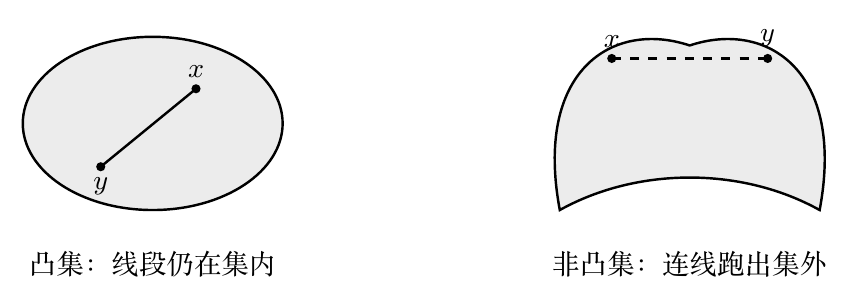
\includegraphics[width=0.92\linewidth]{figs/fig0.png}
\caption{凸集与非凸集}
\end{figure}

凸性是微观理论的“工作假设”：偏好凸保证无差异曲线内弯、技术凸保证边际报酬递减、可行集凸配合极值定理保证最优解“长得规整”。

\subsection{方案空间与可行集}



\textbf{定义 11}\textbf{（方案空间与可行集）}　
设所有潜在方案构成集合 $X$，称为\emph{方案空间}（或选择空间、消费空间）。给定参数 $\theta\in\Theta$，决策者实际能从中选择的方案构成\emph{可行集}
\[
B(\theta)\subseteq X.
\]




可行集\emph{不是}选择结果，而是选择结果可能来自的集合。把二者混同，是初学者最常犯的概念错误之一。

\begin{figure}[H]
\centering
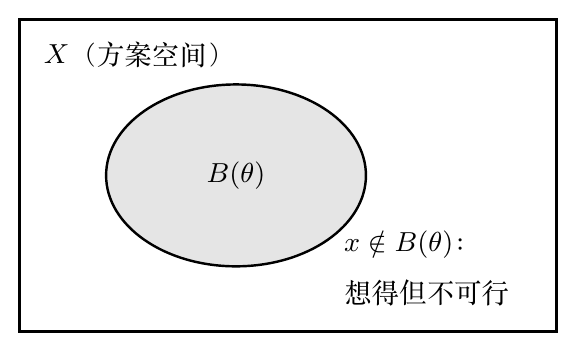
\includegraphics[width=0.92\linewidth]{figs/fig1.png}
\caption{方案空间 $X$ 与可行集 $B(\theta)\subseteq X$}
\end{figure}



\textbf{例 12}\textbf{（预算集）}　
消费例子中，$L$ 种商品的消费束为 $x=(x_1,\dots,x_L)\in X=\R_+^{L}$。给定价格向量 $p\in\R_{++}^{L}$ 与收入 $m\ge 0$，\emph{预算集}为
\[
B(p,m)=\{\,x\in\R_+^{L}: p\cdot x\le m\,\},
\qquad p\cdot x=\sum_{l=1}^{L}p_lx_l .
\]
当 $L=2$ 时，预算线 $p_1x_1+p_2x_2=m$ 在两轴上的截距分别为 $m/p_1$ 与 $m/p_2$，斜率为 $-p_1/p_2$；预算集是预算线左下方的三角形区域（含边界）。




\begin{figure}[H]
\centering
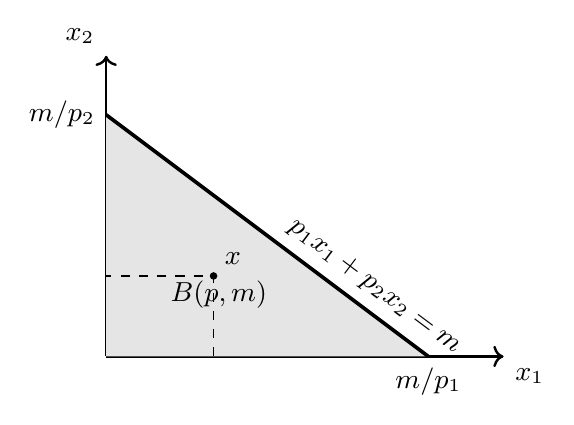
\includegraphics[width=0.92\linewidth]{figs/fig2.png}
\caption{二维预算集：截距、斜率与可行域}
\end{figure}



\textbf{命题 13}\textbf{（预算集的基本性质）}　
设 $p\in\R_{++}^{L}$，$m\ge 0$，则 $B(p,m)$ 是非空、有界、闭且凸的集合。






\emph{证明}　
\textbf{非空}：$0\in B(p,m)$，因 $p\cdot 0=0\le m$。
\textbf{有界}：对 $x\in B(p,m)$，由 $p_l>0$ 与 $x_l\ge 0$ 得 $x_l\le m/p_l$，故 $\lVert x\rVert\le \sqrt{L}\,\max_l(m/p_l)$。
\textbf{闭}：$B(p,m)$ 是闭集 $\{x:p\cdot x\le m\}$ 与闭集 $\R_+^{L}$ 的交，闭集的交仍闭。
\textbf{凸}：任取 $x,y\in B(p,m)$ 与 $\lambda\in[0,1]$，记 $z=\lambda x+(1-\lambda)y$。则 $z_l=\lambda x_l+(1-\lambda)y_l\ge 0$，且
\[
p\cdot z=\lambda\,(p\cdot x)+(1-\lambda)(p\cdot y)\le \lambda m+(1-\lambda)m=m,
\]
故 $z\in B(p,m)$。
　$\square$





\textbf{注 14}　
这个命题值得逐字咀嚼：价格严格为正、收入非负、数量非负——三条看似平淡的假设，恰好保证了下一节要用到的“紧且凸”结构。每一条经济假设都在数学上有明确后果。




\subsection{映射：从方案到数}



\textbf{定义 15}\textbf{（函数）}　
设 $X,Y$ 为两个集合。\emph{函数}（映射）$f:X\to Y$ 是一个规则，使每个 $x\in X$ 对应\emph{唯一}的 $y\in Y$，记 $y=f(x)$。$X$ 称\emph{定义域}，$Y$ 称\emph{值域}（陪域）。




函数有三要素：定义域、值域、对应规则。三者有一个不同，就是不同的函数。



\textbf{定义 16}\textbf{（单射、满射、双射）}　
$f:X\to Y$ 称为\emph{单射}，若 $f(x_1)=f(x_2)\Rightarrow x_1=x_2$；称为\emph{满射}，若对每个 $y\in Y$ 都存在 $x\in X$ 使 $f(x)=y$；既是单射又是满射则称\emph{双射}。






\textbf{例 17}\textbf{（效用是一种映射）}　
在经济学中，映射可以把消费束映为一个实数：
\[
u:X\to\R .
\]
例如 Cobb–Douglas 效用 $u(x_1,x_2)=x_1^{\alpha}x_2^{1-\alpha}$（$0<\alpha<1$），或完全替代效用 $u(x_1,x_2)=a x_1+b x_2$。




这里的 $u(x)$ 是对偏好排序的\emph{数值表示}，而不是方案本身。把方案映到实数，目的是把“更好”转化为可运算的序关系——但这一步骤需要行为假设（理性偏好，见第 5 节），并不等于我们观察到了某种内在的心理单位。



\textbf{注 18}\textbf{（效用的序数性）}　
若 $u$ 表示某偏好，则对任意严格递增变换 $g:\R\to\R$，复合函数 $v=g\circ u$ 表示\emph{同一个}偏好，因为 $u(x)\ge u(y)\iff v(x)\ge v(y)$。所以效用只承载\emph{排序}信息：两个消费束谁更好有意义，“好多少”没有意义。这一“序数性”将在第 6 节评价福利比较时再次出现。






\subsubsection*{本节要点}


\begin{itemize}
  \item 集合语言：$\in,\subseteq,\cup,\cap,\setminus,(\cdot)^{c},\times,\varnothing$；集合相等用双向包含证明；
  \item $\R^{L}$ 中的开/闭、有界、紧、凸——它们分别对应哪些经济含义；
  \item $B(p,m)=\{x\in\R_+^{L}:p\cdot x\le m\}$ 非空、有界、闭、凸（四条逐条可证）；
  \item 函数三要素；效用映射 $u:X\to\R$ 是序数概念。
\end{itemize}

% ==================== 第 3 节：对应（30–50 分钟）====================
\section{从函数到对应}

\subsection{函数与对应的形式差异}



\textbf{定义 19}\textbf{（对应）}　
\emph{对应}（correspondence，又称集值映射）$F:X\rightrightarrows Y$ 是一个规则，使每个 $x\in X$ 对应 $Y$ 的一个\emph{子集} $F(x)\subseteq Y$。




对照函数 $f:X\to Y$（输出一个点），对应 $F:X\rightrightarrows Y$（输出一个集合）。双横箭头 $\rightrightarrows$ 不是装饰：它提醒我们，对应不是“函数写得不够精确”，而是\emph{理论对象本身允许多值}。



\textbf{例 20}　
设 $Y=\{a,b,c\}$，$F(x)=\{a,c\}$。这表示 $a$ 与 $c$ 都是可接受的结果。不能擅自写成 $f(x)=a$——那会丢失“并列”“无差异”或“制度性多解”的信息。




函数是对应的\emph{特殊情形}：若对所有 $x$，$F(x)$ 恰含一个元素，才可以把它视为函数。反向不成立：把多值对象硬写成函数，等于在模型里偷偷加了一条“任意决胜规则”。

\begin{figure}[H]
\centering
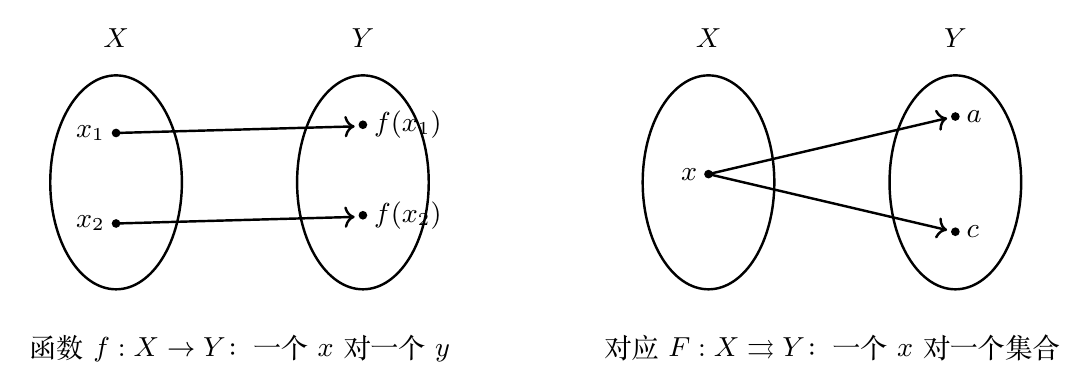
\includegraphics[width=0.92\linewidth]{figs/fig3.png}
\caption{函数与对应：单值输出与集值输出}
\end{figure}

\subsection{选择对应}



\textbf{定义 21}\textbf{（选择对应）}　
给定可行集 $B$，\emph{选择对应}定义为
\[
C(B)\subseteq B,
\]
即从可行集中实际被选出的方案所成的集合。若可行集由参数生成，则写作
\[
C:\Theta\rightrightarrows X,\qquad C(\theta)\subseteq B(\theta).
\]




当多个方案并列最优时，$C(\theta)$ \emph{必须同时包含它们}。



\textbf{例 22}　
设 $B=\{a,b\}$，个体对 $a$ 与 $b$ 无差异，则 $C(B)=\{a,b\}$。若只写 $C(B)=a$，就把理论中的非唯一性错误地替换成了一个任意选择规则——模型于是多了不该有的结论。




\subsection{存在性、唯一性与连续性}

三个性质必须分开问：
\begin{itemize}
  \item \textbf{存在性}：$C(\theta)\neq\varnothing$——“有没有最优解？”
  \item \textbf{唯一性}：$C(\theta)$ 恰含一个元素——“最优解是否只有一个？”
  \item \textbf{连续性}：$\theta$ 微调时 $C(\theta)$ 是否平滑变化——这决定了比较静态是否可靠。
\end{itemize}



\textbf{定理 23}\textbf{（Weierstrass 极值定理）}　
若 $u:X\to\R$ 连续且 $B\subseteq\R^{L}$ 是非空紧集，则 $u$ 在 $B$ 上达到最大值与最小值，即存在 $x^{*}\in B$ 使 $u(x^{*})=\max_{x\in B}u(x)$。因此
\[
\argmax_{x\in B}u(x)\neq\varnothing .
\]






\textbf{例 24}\textbf{（开集上最大值可以不存在）}　
取 $X=\R$，$B=(0,1)$（开区间），$u(x)=x$。$u$ 连续，但 $\sup_{x\in(0,1)}u(x)=1$ 无法达到：对任意 $x\in(0,1)$，总可取 $x'=(x+1)/2>x$。故 $\argmax_{x\in(0,1)}u(x)=\varnothing$。问题正出在 $B$ 不闭，从而不是紧集。






\textbf{注 25}　
连续效用 + 紧致可行集通常只能保证最大值\emph{达到}（存在性），不能保证\emph{唯一}。唯一性需要额外结构：严格凹（或严格拟凹）的目标函数配上凸的可行集，通常带来唯一最优；而线性效用、平坦偏好或非严格凸偏好可能产生\emph{整段}最优解——这正是 $C(\theta)$ 必须是集合而非点的第二个理由（第一个理由是无差异）。






\subsubsection*{本节要点}


\begin{itemize}
  \item $f:X\to Y$ 输出点，$F:X\rightrightarrows Y$ 输出子集；函数是对应的特例；
  \item 选择对应 $C(\theta)\subseteq B(\theta)$ 天生是集值对象；
  \item 存在性靠“连续 + 紧”，唯一性靠“严格凹 + 凸”，二者不可混淆；
  \item 反例：开区间上的线性函数没有最大值。
\end{itemize}

% ==================== 第 4 节：参数与选择（50–70 分钟）====================
\section{参数、可行集与最优选择}

\subsection{参数如何决定可行集}

参数不是模型外的装饰，而是决定机会集合形状的\emph{输入}。一般写作
\[
B:\Theta\rightrightarrows X,\qquad \theta=(p,m,\tau,\omega,\dots),
\]
其中 $\tau$ 可代表税率或补贴，$\omega$ 可代表禀赋。价格与收入决定预算约束；税收可能改变斜率、截距或可行域的分段结构；配额会直接“切掉”一部分集合。

\begin{figure}[H]
\centering
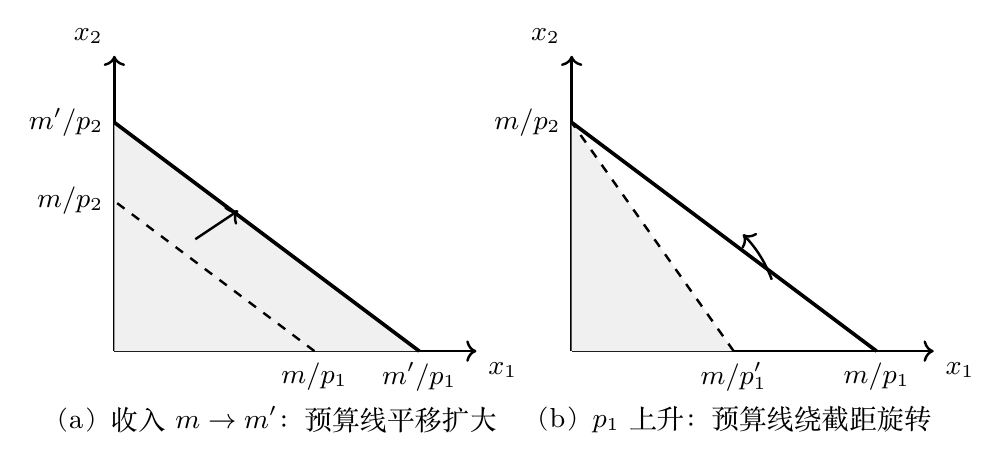
\includegraphics[width=0.92\linewidth]{figs/fig4.png}
\caption{参数变化如何改变可行集：平移与旋转}
\end{figure}



\textbf{注 26}　
收入变化与价格变化对 $B(p,m)$ 的作用在几何上完全不同：$m$ 只改截距不改斜率（机会成本不变）；$p_1/p_2$ 改变斜率（相对价格即机会成本），同时改变一个截距。比较静态的第一步永远是：\emph{哪个参数变了？它怎么改变可行集？}




\subsection{最优选择的两种输出：\texorpdfstring{$C(\theta)$}{C(θ)} 与 \texorpdfstring{$v(\theta)$}{v(θ)}}

若偏好可由效用函数 $u:X\to\R$ 表示，则选择对应为
\[
\boxed{\,C(\theta)=\argmax\{\,u(x):x\in B(\theta)\,\}\,}
\]

逐字解释：
\begin{itemize}
  \item $C(\theta)$：参数为 $\theta$ 时的\emph{所有}最优方案（一个集合）；
  \item $\argmax$：取的是“使目标达到最大值的\emph{自变量}集合”，而不是最大值本身；
  \item $u(x)$：目标函数；
  \item $x\in B(\theta)$：只能在参数决定的可行集中选择。
\end{itemize}

必须严格区别：
\[
v(\theta)=\max_{x\in B(\theta)}u(x)\in\R
\qquad\text{与}\qquad
C(\theta)=\{\,x\in B(\theta):u(x)=v(\theta)\,\}\subseteq X .
\]
$v(\theta)$ 是\emph{最大值函数}（indirect utility，间接效用），输出一个\emph{数}；$C(\theta)$ 输出达到该数的\emph{所有方案}。最大值回答“最高能达到多少”，argmax 回答“哪些方案达到最高”。

\begin{figure}[H]
\centering
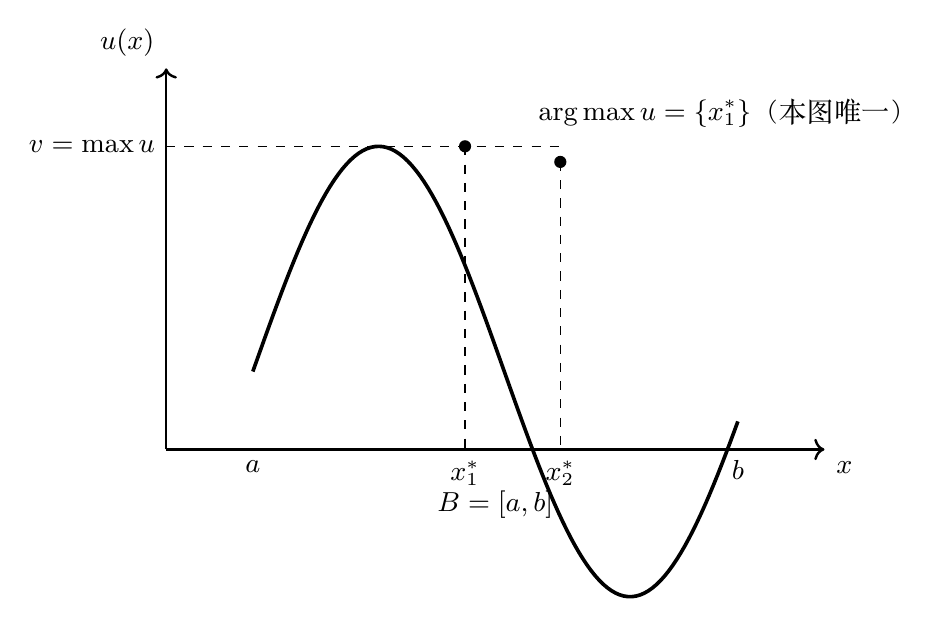
\includegraphics[width=0.92\linewidth]{figs/fig5.png}
\caption{最大值 $v$ 是一个数；$\argmax$ 是达到它的自变量集合}
\end{figure}



\textbf{例 27}\textbf{（数值对照）}　
设 $B=[0,4]$，$u(x)=-(x-2)^2+5$。则 $v=\max u=5$（一个数），$C=\argmax u=\{2\}$（一个集合，本例为单点集）。若改为 $u(x)=\min\{x,2\}$，则 $v=2$ 而 $C=[2,4]$——\emph{整段}都是最优解。




\subsection{为什么 \texorpdfstring{$C(\theta)$}{C(θ)} 必须允许是集合}

第 3 节已给出理由（无差异）。第二个经典来源是\emph{线性效用}：设 $u(x_1,x_2)=x_1+x_2$，$p=(1,1)$，$m=1$。预算线为 $x_1+x_2=1$，效用线与其斜率相同，故预算线上\emph{每一点}都是最优：
\[
C(p,m)=\{\,(x_1,x_2)\in\R_+^2:x_1+x_2=1\,\},
\]
一条线段，而不是一个点。

\begin{figure}[H]
\centering
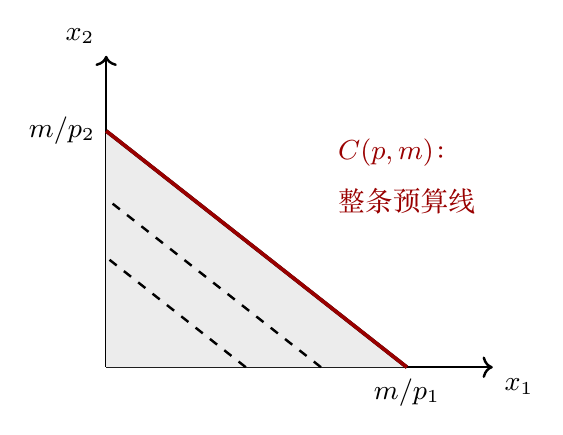
\includegraphics[width=0.92\linewidth]{figs/fig6.png}
\caption{线性效用与预算线斜率相同：最优解是\emph{一整段}集合}
\end{figure}

\subsection{比较静态}



\textbf{定义 28}\textbf{（比较静态）}　
比较静态（comparative statics）研究参数 $\theta$ 变化如何引起 $B(\theta)$、$C(\theta)$ 或 $v(\theta)$ 的变化。形式上，若 $v$ 可微，则
\[
\mathrm{d}v=\sum_{k}\frac{\partial v}{\partial\theta_k}\,\mathrm{d}\theta_k .
\]






\textbf{例 29}\textbf{（收入效应的符号）}　
在正规品假设下，$\partial x_l^{*}/\partial m>0$：收入上升，需求上升。这是一条\emph{可检验}的比较静态命题——第 6 节会看到，这类命题正是实证研究的典型产出。






\textbf{注 30}\textbf{（比较静态 $\neq$ 因果识别）}　
比较静态给出的是\emph{模型内}结论：“保持其他结构不变，$\theta$ 变，则 $C$ 变”。若现实中价格变化同时携带信息、预期或制度变化，结构解释还需额外假设。博士生应始终追问三问：改变的是哪个原语（primitive）？保持了哪些条件？结论对替代参数化是否稳健？




\begin{figure}[H]
\centering
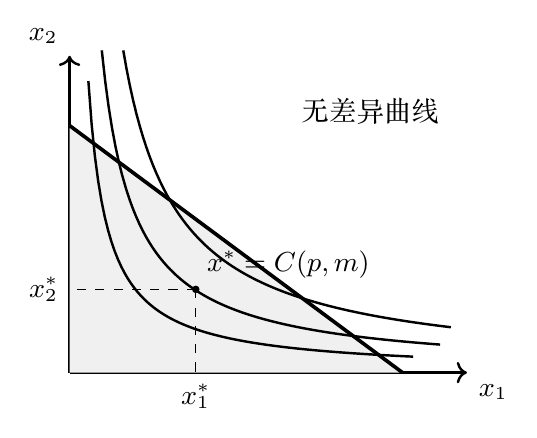
\includegraphics[width=0.92\linewidth]{figs/fig7.png}
\caption{内点最优：无差异曲线与预算线相切于 $x^{*}$}
\end{figure}



\subsubsection*{本节要点}


\begin{itemize}
  \item $v(\theta)\in\R$ 是数，$C(\theta)\subseteq X$ 是集合——输出类型不同，不可混写；
  \item $\argmax$ 取“使目标最大的自变量集合”；
  \item 线性效用、平坦偏好 $\Rightarrow$ $C(\theta)$ 可以是一整段；
  \item 比较静态三问：改什么、保什么、是否稳健。
\end{itemize}

% ==================== 第 5 节：纯选择理论（70–85 分钟）====================
\section{纯选择理论：不预设目标函数}

\subsection{公理化起点：只规定选择对应}

抽象选择理论从\emph{可观察的选择事实}出发，只规定三样东西：
\[
X\ (\text{方案空间}),\qquad \mathcal{B}\ (\text{可行集的族}),\qquad C(B)\subseteq B\ (\text{选择对应}),
\]
而\emph{不必先给定}效用函数 $u$。

\subsection{为什么可以不预设 \texorpdfstring{$u$}{u}}

至少有四条理由：
\begin{enumerate}
  \item \textbf{目标函数可能不可观察}。我们能记录“选了什么”，但看不到“为什么”。
  \item \textbf{行为可能由非最优化机制产生}。程序、注意力、社会规范、有限理性都可能生成选择。
  \item \textbf{选择可能循环}。若 $a$ 胜 $b$、$b$ 胜 $c$、$c$ 又胜 $a$，则不存在传递偏好可以理性化这些选择。
  \item \textbf{识别不唯一}。即使存在效用表示，数据也未必能唯一识别它（序数效用的单调变换无穷多）。
\end{enumerate}

因此，“存在某个 $u$ 使 $C(B)=\argmax_{x\in B}u(x)$”是一个\emph{待检验、待证明的理性化命题}，而不是逻辑起点。



\textbf{定义 31}\textbf{（理性化）}　
称偏好关系 $\succeq$ \emph{理性化}（rationalize）选择对应 $C$，若对每个可行集 $B$，
\[
C(B)=\{\,x\in B : x\succeq y,\ \forall\, y\in B\,\}.
\]




\subsection{显示偏好与一致性条件}

显示偏好理论的核心思想是：从\emph{不同预算集}中的实际选择，检验是否存在一个统一偏好关系可以解释全部选择。



\textbf{定义 32}\textbf{（直接显示偏好）}　
若 $x$ 在 $y$ 可行时被选择（即 $y\in B$ 而 $x\in C(B)$），称 $x$ \emph{直接显示偏好于} $y$，记 $x\succeq^{R}y$。






\textbf{条件 33}\textbf{（WARP，显示偏好弱公理）}　
若 $x\succeq^{R}y$ 且 $x\neq y$，则不可能有 $y\succeq^{R}x$。换言之：若 $x$ 在 $y$ 买得起时被选中，那么当 $y$ 被选中时，$x$ 必定\emph{买不起}。






\textbf{例 34}\textbf{（违反 WARP 的选择）}　
设 $B_1=\{a,b\}$，观察得 $C(B_1)=\{a\}$（故 $a\succeq^{R}b$）。又设 $B_2=\{a,b,c\}$，若观察得 $b\in C(B_2)$ 而 $a$ 也可行，则 $b\succeq^{R}a$，与 $a\succeq^{R}b$ 矛盾——这组选择不能被任何理性偏好解释。




把 WARP 加强为沿“显示偏好链”的一致性，即得 \textbf{SARP}（显示偏好强公理）：若 $x_1\succeq^{R}x_2\succeq^{R}\cdots\succeq^{R}x_n$ 且 $x_1\neq x_n$，则不能有 $x_n\succeq^{R}x_1$。Afriat 定理表明：满足 SARP 的有限选择数据，必可被某个单调、连续、凹的效用函数理性化——\emph{理性化问题从而有了可检验的答案}。

\begin{figure}[H]
\centering
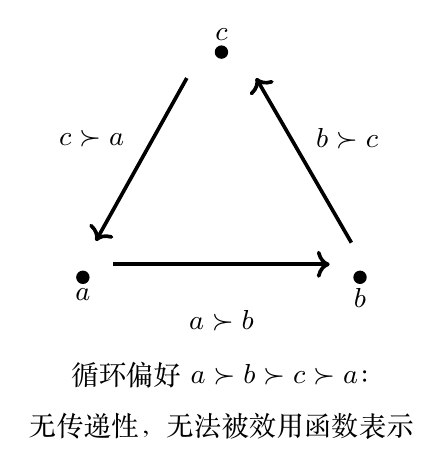
\includegraphics[width=0.92\linewidth]{figs/fig8.png}
\caption{循环选择：理性化失败的典型反例}
\end{figure}

\subsection{不预设目标函数 ≠ 否认行为规律}

不预设 $u$，只是\emph{把解释任务后移}：先让数据说话，再问何种偏好（如果存在）能解释它。这是理论经济学的方法论自觉——模型应当对“可观察的不一致”保持敏感，而不是用数学形式掩盖它。



\subsubsection*{本节要点}


\begin{itemize}
  \item 纯选择理论只给 $C(B)\subseteq B$，不预设 $u$；
  \item “$C$ 可被效用理性化”是定理/检验的结论，不是公理；
  \item 直接显示偏好 $\succeq^{R}$、WARP、SARP 构成可检验的一致性阶梯；
  \item 循环偏好 $a\succ b\succ c\succ a$ 是理性化失败的最小反例。
\end{itemize}

% ==================== 第 6 节：实证与规范（85–102 分钟）====================
\section{实证分析与规范分析：两种不同的问题}

经济学研究常被混作一谈的两类问题，其实属于不同的逻辑类别：\emph{实证}（positive）研究“是什么”，\emph{规范}（normative）研究“应当怎样”。把二者分开，是博士生必须具备的方法论基本功。

\subsection{实证分析：回答“是什么”}



\textbf{定义 35}\textbf{（实证命题）}　
\emph{实证命题}是关于世界\emph{是}什么样、以及“若……则……”会怎样变化的可检验陈述。它回答三类问题：是什么（描述）、为什么（机制）、会怎样（预测）。




实证命题的三个特征：
\begin{enumerate}
  \item \textbf{概念清晰}：每个术语都有可操作的定义（如“正常品”定义为 $\partial x_l^{*}/\partial m>0$）；
  \item \textbf{机制明确}：因果链条在模型内部可追踪（$\theta\to B(\theta)\to C(\theta)$）；
  \item \textbf{预测可检验}：原则上存在数据可以\emph{推翻}它。
\end{enumerate}



\textbf{例 36}\textbf{（比较静态是典型实证命题）}　
“收入增加会提高对正常品的需求”——在保持偏好、价格不变且满足假设 $A$ 时，参数 $m$ 的上升导致选择集合发生特定变化：
\[
m'\ge m \;\Longrightarrow\; x_l^{*}(p,m')\ge x_l^{*}(p,m)\quad(\text{正常品}).
\]
又如：“税率 $\tau$ 上升会降低劳动供给”——这是关于 $C(\theta)$ 对 $\tau$ 的比较静态，原则上可用微观数据检验。




实证结论的规范写法是带\emph{条件}的：
\[
\text{在保持 }Z\text{ 不变且满足假设 }A\text{ 时，参数 }p\text{ 的变化导致选择发生某种变化。}
\]
丢掉条件，实证命题就从“可检验”退化为“口号”。

\subsection{规范分析：回答“应当怎样”}



\textbf{定义 37}\textbf{（规范命题）}　
\emph{规范命题}是关于“什么应当发生”“哪个结果更好”的陈述。它必须援引某个\emph{价值标准}（福利准则），而价值标准不能从事实中自动推出。




最常用的价值标准有：
\begin{itemize}
  \item \textbf{帕累托标准}：状态 $x$ 帕累托优于 $y$，若无人变差且至少一人变好（严格写法见下）。帕累托改进得到的是\emph{效率}判断，不涉及分配；
  \item \textbf{功利主义社会福利函数}：
        \[
        W(u_1,\dots,u_n)=\sum_{i=1}^{n}\alpha_i u_i,\qquad \alpha_i\ge 0,
        \]
        把社会评价写成个体效用的加权和；
  \item \textbf{罗尔斯（max–min）标准}：$W=\min_i u_i$，社会评价取决于最不利者。
\end{itemize}



\textbf{注 38}\textbf{（权重不是事实）}　
功利主义中的权重 $\alpha_i$ \emph{不是}由个体选择事实自动推出的，它体现的是评价者的价值立场（谁更重要）。把某个 $\alpha$ 当作“客观的”，正是把规范伪装成实证。同理，效率提高不意味公平改善；观察到某政策“有效”，也不等于该政策“正当”。






\textbf{定义 39}\textbf{（帕累托最优）}　
配置 $x$ 称为\emph{帕累托最优}（Pareto optimal），若不存在其他可行配置 $x'$ 使所有人 $i$ 满足 $u_i(x'_i)\ge u_i(x_i)$ 且至少一个 $j$ 满足 $u_j(x'_j)>u_j(x_j)$。






\textbf{例 40}\textbf{（效率与公平可以背离）}　
把所有资源给一个人而其余人为零，可以是帕累托最优（无法在不损害该人的前提下改善他人），但几乎无人认为它“应当”如此。帕累托标准对分配沉默，这正是它作为\emph{最低限度}价值标准的原因与局限。




\subsection{三层分离}

政策评价应分三层进行：

\begin{figure}[H]
\centering

\includegraphics[width=0.92\linewidth]{figs/fig9.png}
\caption{政策评价的三层分离}
\end{figure}



\textbf{注 41}　
把第三层（价值）伪装成第一层（事实），是经济学论证中最常见的越界。例如“最低工资提高了效率，所以应该实行最低工资”——前半句即使有证据，后半句仍需额外的价值前提才能成立。




\subsection{案例演练：把一个政策问题拆成正反两半}

\begin{center}
\small
\begin{tabular}{p{2.6cm}p{5.6cm}p{5.6cm}}
\toprule
政策 & 实证命题（是什么） & 规范判断（应当怎样） \\
\midrule
最低工资 & 提高最低工资降低低技能工人的就业量（弹性可估计） & 应当/不应当实行最低工资（需福利标准与分配权重） \\
房产税 & 开征房产税降低投资性购房需求、改变地方财政收入结构 & 应当/不应当开征（效率与公平的权衡是价值问题） \\
消费券/补贴 & 消费券在短期内提高边际消费倾向高的群体的消费 & 应当/不应当发放（跨期效率、财政成本与目标人群是价值判断） \\
\bottomrule
\end{tabular}
\end{center}

注意左栏每一条原则上都可被数据\emph{证伪}；右栏每一条都必须明示其价值标准。两栏不可互相替代。

\subsection{实证与规范的互补}

实证与规范不是对手，而是完整研究的两个半部：
\[
\underbrace{\text{实证：预测政策后果}}_{\text{没有它，规范是空中楼阁}}
\;+\;
\underbrace{\text{规范：评价后果好坏}}_{\text{没有它，实证无政策含义}}
\;\Longrightarrow\; \text{完整的政策分析}.
\]
实证错误会让规范结论建立在沙上；规范模糊会让实证研究失去方向。博士生的写作规范是：每一段都先说清楚自己在哪一层。



\subsubsection*{本节要点}


\begin{itemize}
  \item 实证：是什么/为什么/会怎样；三特征——概念清晰、机制明确、可检验；
  \item 规范：应当怎样；必须援引价值标准（帕累托、功利主义 $W=\sum\alpha_i u_i$、罗尔斯）；
  \item 权重 $\alpha_i$ 是价值立场而非事实；效率 $\neq$ 公平；
  \item 三层分离：事实层、机制层、价值层；越界是最常见错误。
\end{itemize}

% ==================== 第 7 节：模型价值（102–115 分钟）====================
\section{模型的价值与适用边界}

一个好模型不是“更复杂”或“更现实”的模型。本节给出六个评价维度，并说明它们之间的张力。

\subsection{六维评价框架}

\begin{center}
\small
\begin{tabular}{p{2.6cm}p{4.3cm}p{4.2cm}p{3.4cm}}
\toprule
维度 & 核心问题 & 证据 & 主要风险 \\
\midrule
Useful 有用 & 能回答重要问题吗？ & 解释、政策用途、反事实 & 问题选择过窄 \\
Accurate 准确 & 预测与数据一致吗？ & 样本外预测、实验与准实验 & 过拟合 \\
Broad 广泛 & 能迁移到其他场景吗？ & 消费、生产、劳动等应用 & 过宽而不可证伪 \\
Compact 简洁 & 以少量结构产生清晰推论？ & 假设–结论压缩比 & 忽略关键机制 \\
Identifiable 可识别 & 参数能被数据区分吗？ & 识别策略、敏感性分析 & 依赖不可观测假设 \\
Falsifiable 可证伪 & 什么结果会推翻它？ & 明确反事实与拒绝条件 & 模型永远可解释 \\
\bottomrule
\end{tabular}
\end{center}

\subsection{逐维展开}



\subsubsection*{7.2.1 Useful：有用而非万能}


模型的有用性取决于\emph{问题}。选择模型能从选择恢复偏好、组织制度比较，并与个体自主性相容；但人际效用比较困难——不能把个体内部的序数排序直接加总为社会福利（这正是第 6 节 $W$ 需要外生权重的根源）。



\subsubsection*{7.2.2 Accurate：准确必须指向可检验含义}


一个模型不是因为数学精致就准确。应区分四种“准确”：样本内拟合、样本外预测、结构参数识别、反事实有效性。比较静态只有在参数具有清晰制度含义、且其他机制被控制时，才有经验内容。



\subsubsection*{7.2.3 Broad 与 Compact 的张力}


越宽泛的模型越可能迁移，但越难产生锐利预测；越紧凑的模型越便于推导，却可能忽略注意力、身份、规范与非传递性。简化本身不是缺陷，关键是明确回答：\emph{为了哪个问题，牺牲了哪些现实因素？}



\subsubsection*{7.2.4 Identifiable：参数能否被数据区分}


若两组截然不同的参数 $(\theta_1,\theta_2)$ 产生完全相同的选择数据，则该参数不可识别。识别失败时，一切“结构解释”都是空中楼阁。补救办法：补充数据维度、施加可辩护的约束、或改问可识别的问题。



\subsubsection*{7.2.5 Falsifiable：必须说清什么会推翻它}


一个“无论看到什么都能解释”的模型没有信息量。写模型时就应写下拒绝条件：若数据呈现 $X$，则放弃该模型。可证伪性是把实证研究与讲故事区分开的底线。

\subsection{简化假设、反例与边界}

经典选择框架的最小假设可表述为：
\begin{enumerate}
  \item 选择来自某个可行集；
  \item 被偏好的方案更可能被选择；
  \item 任意两个潜在方案可以比较（完全性）；
  \item 偏好具有传递性。
\end{enumerate}

每一条假设都应对应一个\emph{结论依赖点}和一个\emph{最小反例}：
\begin{itemize}
  \item 删除\emph{完全性} $\Rightarrow$ 某些方案无法比较，$C(B)$ 可能无法定义；
  \item 删除\emph{传递性} $\Rightarrow$ 可能出现 $a\succ b\succ c\succ a$ 的循环，无法被效用表示；
  \item 删除\emph{紧致性} $\Rightarrow$ 最大值可能不存在（开区间上的线性函数）；
  \item 删除\emph{严格凹性} $\Rightarrow$ 最优方案可能不唯一（线性效用）。
\end{itemize}



\subsubsection*{边界声明的写法}


好的论文在模型之后紧跟一段“边界声明”：本模型在哪些条件下成立、哪些机制被有意忽略、哪些结论对哪些假设敏感。这不是示弱，而是把模型的\emph{适用范围}写清楚——它恰恰是可信度的来源。



\subsubsection*{本节要点}


\begin{itemize}
  \item 六维评价：Useful、Accurate、Broad、Compact、Identifiable、Falsifiable；
  \item Broad 与 Compact 存在张力；Accurate 必须指向可检验含义；
  \item 每条假设对应一个结论依赖点 + 一个最小反例；
  \item 边界声明是模型可信度的一部分。
\end{itemize}

% ==================== 第 8 节：总结、测验与作业（115–120 分钟）====================
\section{总结、课堂测验与作业}

\subsection{一条逻辑链}

本讲的核心不是“把一切行为都写成最大化”，而是理解一连串\emph{逻辑转换的条件}：
\[
\underbrace{X\supseteq B(\theta)}_{\text{从方案到可行集}}
\;\longrightarrow\;
\underbrace{C(\theta)\subseteq B(\theta)}_{\text{从可行集到选择}}
\;\longrightarrow\;
\underbrace{\succeq^{R}}_{\text{从选择到偏好}}
\;\longrightarrow\;
\underbrace{u:X\to\R}_{\text{从偏好到效用}}
\;\longrightarrow\;
\underbrace{C(\theta)=\argmax_{x\in B(\theta)}u(x)}_{\text{从效用表达到优化}},
\]
压缩成一句话：
\[
\text{choice data}\;\Rightarrow\;\text{preference representation}\;\Rightarrow\;\text{optimization}\;\Rightarrow\;\text{testable implications}.
\]

\subsection{三个必须记住的反例}
\begin{enumerate}
  \item \textbf{非唯一最优}：$u(x_1,x_2)=x_1+x_2$，$p=(1,1)$，$m=1$ 时 $C(p,m)$ 是整条预算线——故选择对应\emph{必须}是集值对象；
  \item \textbf{最大值不存在}：$B=(0,1)$、$u(x)=x$ 时 $\argmax=\varnothing$——存在性依赖紧致性；
  \item \textbf{循环偏好}：$a\succ b\succ c\succ a$——传递性缺失时无法被效用理性化。
\end{enumerate}

\subsection{课堂测验（5 分钟）}
\begin{enumerate}
  \item 若两个消费束都达到最大效用，为什么不能把选择对应写成函数？\\
        \emph{要点：}函数要求唯一输出；并列最优意味着输出含两个元素，写成函数等于偷偷加入任意决胜规则，丢失无差异信息。
  \item $v(\theta)$ 与 $C(\theta)$ 的输出类型分别是什么？\\
        \emph{要点：}$v(\theta)=\max u\in\R$ 是数；$C(\theta)=\argmax u\subseteq X$ 是集合。
  \item 预算线移动时，变化的是偏好还是可行集？\\
        \emph{要点：}可行集 $B(\theta)$。偏好 $\succeq$ 是行为原语，不随参数变化；这是比较静态的前提。
  \item “税收提高效率”为什么还不足以推出“税收应当提高”？\\
        \emph{要点：}前者是实证命题（事实层），后者是规范判断（价值层），需要额外福利标准才能连接。
  \item 一个模型越现实是否一定越有价值？\\
        \emph{要点：}否。Broad 与 Compact 存在张力；价值取决于六维综合表现与所回答的问题。
\end{enumerate}

\subsection{课后作业}
\begin{enumerate}
  \item 构造一个最小例子，使 $\argmax$ 恰好含有\emph{两个}元素，并画出图形；
  \item 给出一个没有最大值的可行集与连续目标函数（不得照抄课堂反例），并说明缺少的是哪一条性质；
  \item 用预算集解释收入效应与替代效应的逻辑区别（提示：先分解“哪个参数变了”）；
  \item 选择一个你关心的政策模型，分别写出它的：正向命题、规范标准、识别风险与可证伪条件。
\end{enumerate}

\subsection{结语}

最终评价一个模型时，应同时追问：它是否\emph{有用}、是否\emph{准确}、是否足够\emph{广泛}、是否保持\emph{简洁}、是否\emph{可识别}、是否\emph{可证伪}，以及它的规范结论究竟依赖了哪些价值前提。把这六问变成肌肉记忆，是本课最重要的产出。


% ==================== 参考文献 ====================

\section*{参考文献}
\begin{enumerate}
  \item Arrow, K. J. (1951). \emph{Social Choice and Individual Values}. Yale University Press.
  \item Debreu, G. (1959). \emph{Theory of Value}. Wiley.
  \item Afriat, S. N. (1967). The construction of separable utility functions from expenditure data. \emph{International Economic Review}, 8(1), 67–77.
  \item Sen, A. (1970). \emph{Collective Choice and Social Welfare}. Holden-Day.
  \item Varian, H. R. (1992). \emph{Microeconomic Analysis} (3rd ed.). Norton.
  \item Hausman, D. M. (1992). \emph{The Inexact and Separate Science of Economics}. Cambridge University Press.
  \item Mas-Colell, A., Whinston, M. D., \& Green, J. R. (1995). \emph{Microeconomic Theory}. Oxford University Press.
\end{enumerate}

